
\documentclass[12pt]{article}
\usepackage[english]{babel}
\usepackage{t1enc}

% AMS packages:
\usepackage{amsbsy}
\usepackage{amsfonts}
\usepackage{amsmath}
\usepackage{amssymb}
\usepackage{amsthm}
\usepackage{amsxtra}
\usepackage{graphicx}
\usepackage{bbm}
% for comments to work
\usepackage{verbatim}
\usepackage{hyperref}

%%%%%%%%%%%%%%%%%%%%%%%%%%%%%%%%%%%

% Hilbert spaces:
\newcommand{\hilb}{\mathcal{H}}
\newcommand{\banH}{\mathcal{B}(\hilb)}
\newcommand{\fock}{\mathcal{F}}

% Products:
\newcommand{\scalpr}[2]{( #1, #2 )}
\newcommand{\dualpr}[2]{\langle #1, #2 \rangle}

% Fonts
\newcommand{\calc}{\mathcal{C}}
\newcommand{\cala}{\mathcal{A}}
\newcommand{\calv}{\mathcal{V}}
\newcommand{\calf}{\mathcal{F}}
\newcommand{\cals}{\mathcal{S}}
\newcommand{\cald}{\mathcal{D}}
\newcommand{\banach}{\mathcal{B}}
\newcommand{\id}[1]{\mathbbm{1}\!\left({#1}\right)}

\newcommand{\ci}{{\rm i}}
\newcommand{\rmd}{{\rm d}}
\newcommand{\rme}{{\rm e}}

\newcommand{\re}{{\rm Re\,}}
\newcommand{\im}{{\rm Im\,}}

% misc
\newcommand{\defem}[1]{{\em #1\/}}
\newcommand{\vep}{\varepsilon}


\newcommand{\qand}{\quad\text{and}\quad}

% To define sets:
\newcommand{\defset}[2]{ \left\{ #1 \left|\, #2\makebox[0pt]{$\displaystyle\phantom{#1}$}\right.\!\right\} }

\newcounter{alplisti}
\renewcommand{\thealplisti}{\alph{alplisti}}
\newenvironment{alplist}[1][(\thealplisti)]{\begin{list}{{\rm #1}\ }{ %
      \usecounter{alplisti} %
    \setlength{\itemsep}{0pt}
    \setlength{\parsep}{0pt}  %
%    \setlength{\leftmargin}{5em} %
%    \setlength{\labelwidth}{5em} %
%    \setlength{\labelsep}{1em} %
%    \settowidth{\labelwidth}{(DR2)}
     \setlength{\topsep}{0pt} %
}}{\end{list}}

% Norms:
\newcommand{\abs}[1] {\lvert #1 \rvert}
\newcommand{\norm}[1]{\lVert #1 \rVert}
\newcommand{\floor}[1] {\lfloor {#1} \rfloor}
\newcommand{\ceil}[1]  {\lceil  {#1} \rceil}

% Basic spaces
\newcommand{\R} {\mathbb{R}}
\newcommand{\C} {{\mathbb{C}}}
\newcommand{\Rd} {{\mathbb{R}^{d}}}
\newcommand{\N} {\mathbb{N}}
\newcommand{\Z} {\mathbb{Z}}
\newcommand{\Q} {\mathbb{Q}}
\newcommand{\K} {\mathbb{K}}
\newcommand{\T} {\mathbb{T}}

%%%%%%%%%%%%%%%%%%%%%%%%%%%%%%%%%%%


\newcommand{\pat}{\partial}
\newcommand{\be}{\begin{equation}}
\newcommand{\ee}{\end{equation}}
\newcommand{\bea}{\begin{eqnarray}}
\newcommand{\eea}{\end{eqnarray}}
\newcommand{\abf}{{\bf a}}
\newcommand{\Zcal}{{\cal Z}_{12}}
\newcommand{\zcal}{z_{12}}
\newcommand{\Acal}{{\cal A}}
\newcommand{\Fcal}{{\cal F}}
\newcommand{\Ucal}{{\cal U}}
\newcommand{\Vcal}{{\cal V}}
\newcommand{\Ocal}{{\cal O}}
\newcommand{\Rcal}{{\cal R}}
\newcommand{\Scal}{{\cal S}}
\newcommand{\Lcal}{{\cal L}}
\newcommand{\Hcal}{{\cal H}}
\newcommand{\hsf}{{\sf h}}
\newcommand{\half}{\frac{1}{2}}
\newcommand{\Xbar}{\bar{X}}
\newcommand{\xibar}{\bar{\xi }}
\newcommand{\barh}{\bar{h}}
\newcommand{\Ubar}{\bar{\cal U}}
\newcommand{\Vbar}{\bar{\cal V}}
\newcommand{\Fbar}{\bar{F}}
\newcommand{\zbar}{\bar{z}}
\newcommand{\wbar}{\bar{w}}
\newcommand{\zbarhat}{\hat{\bar{z}}}
\newcommand{\wbarhat}{\hat{\bar{w}}}
\newcommand{\wbartilde}{\tilde{\bar{w}}}
\newcommand{\barone}{\bar{1}}
\newcommand{\bartwo}{\bar{2}}
\newcommand{\nbyn}{N \times N}
\newcommand{\repres}{\leftrightarrow}
\newcommand{\Tr}{{\rm Tr}}
\newcommand{\tr}{{\rm tr}}
\newcommand{\ninfty}{N \rightarrow \infty}
\newcommand{\unitk}{{\bf 1}_k}
\newcommand{\unitm}{{\bf 1}}
\newcommand{\zerom}{{\bf 0}}
\newcommand{\unittwo}{{\bf 1}_2}
\newcommand{\holo}{{\cal U}}
\newcommand{\bra}{\langle}
\newcommand{\ket}{\rangle}
\newcommand{\muhat}{\hat{\mu}}
\newcommand{\nuhat}{\hat{\nu}}
\newcommand{\rhat}{\hat{r}}
\newcommand{\phat}{\hat{\phi}}
\newcommand{\that}{\hat{t}}
\newcommand{\shat}{\hat{s}}
\newcommand{\zhat}{\hat{z}}
\newcommand{\what}{\hat{w}}
\newcommand{\sgamma}{\sqrt{\gamma}}
\newcommand{\bfE}{{\bf E}}
\newcommand{\bfB}{{\bf B}}
\newcommand{\bfM}{{\bf M}}
\newcommand{\cl} {\cal l}
\newcommand{\ctilde}{\tilde{\chi}}
\newcommand{\ttilde}{\tilde{t}}
\newcommand{\ptilde}{\tilde{\phi}}
\newcommand{\utilde}{\tilde{u}}
\newcommand{\vtilde}{\tilde{v}}
\newcommand{\wtilde}{\tilde{w}}
\newcommand{\ztilde}{\tilde{z}}

\selectlanguage{english}

\hoffset 0.5cm
\voffset -0.4cm
\evensidemargin -0.2in
\oddsidemargin -0.2in
\topmargin -0.2in
\textwidth 6.3in
\textheight 8.4in

\begin{document}

\normalsize

\baselineskip 14pt

\begin{center}
{\Large {\bf FYMM/MMP III \ \ \   Solutions to Problem Set 2}}
\\
{\large{Jake Muff}}
\\
10/9/20
\end{center}


\begin{enumerate}
\item Question 1
\\ 
To be a group iosmorphism two groups need to have group homomorphism i.e 
$$ g_1 g_2 \in G, f(g_1 g_2) =f(g_1)f(g_2) $$
And map $f$ is also a bijection, requiring that $f$ is injective and surjective i.e $f \rightarrow$ one to one mapping and $f \rightarrow $ maps onto. 
\\ So, define the mappings: $f:M(n,\mathbb{R}) \rightarrow \mathbb{R}^{n^2}$:
$$ \left( \begin{array}{cccc} a_{11} & a_{12} & \ldots & a_{1n} \\ a_{21} &  & & \\ \vdots &  & & \\ a_{n1} & a_{n2} & \ldots & a_{nn} \end{array}\right) \rightarrow (a_{11} \ldots a_{1n}, a_{21} \ldots a_{n1}, a_{nn})$$
And $g: \mathbb{R}^{n^2} \rightarrow M(n,\mathbb{R})$
$$ (x_1 \ldots x_n^2) \rightarrow \left( \begin{array}{cccc} x_{1} & x_{2} & \ldots & x_{n} \\ x_{n+1} &  & & \\ \vdots &  & & \\ x_{n^2-n+1} & \ldots & \ldots & x_{n^2} \end{array}\right) $$
We see that $f$ has one to one mapping as well as the product between $g$ and $f$ creating an identity matrix the size of $\mathbb{R}^{n^2}$. 
\\
We also see that $f$ is mapping $M(n,\mathbb{R})$ onto $\mathbb{R}^{n^2}$ and is surjective with the product between $f$ and $g$ being equal to an identity matrix of size $M(n,\mathbb{R})$, showing that $f$ is a bijection. 
\\ 
To show a group homomorphism:
$$ f(h \circ i) = f\left( \begin{array}{cccc} h_{11}+i_{11} & h_{12}+i_{12} & \ldots & h_{1n}+i_{1n} \\ h_{21}+i_{21} &  & & \\ \vdots &  & & \\ h_{n1}+i_{n1} & \ldots & \ldots & h_{nn}+i_{nn} \end{array}\right) $$
Which from the above maps is equal to: 
$$ (h_{11}+i_{11} \ldots h_{1n}+i_{1n}, h_{21}+i_{21} \ldots h_{2n}+i_{2n} \ldots h_{n1}+i_{n1} \ldots h_{nn}+i_{nn}) $$
Which is $ = h \circ i \ \circ : \mathbb{R}^{n^2} $
\\ 
Therefore $f:M(n,\mathbb{R}^{n^2}) \rightarrow \mathbb{R}^{n^2}$ is both bijective and group homomorphism so we can say that $M(n,\mathbb{R}^{n^2}) \cong \mathbb{R}^{n^2} $


\item Question 2
\\ For these multiplication I effectively use matrix multiplications using the matrix forms of the permutation groups and taking the reverse i.e 
\begin{itemize}
\item $$ (235)(46)\cdot(14)(265) $$
$$ = M((14)/cdot(265)) /cdot M((235)/cdot(46)) $$
Where the $M$ represents the matrix form of the permutation. I then reverse the matrix given into simple one line notation.
$$ (235)(46)\cdot(14)(265) $$
$$ \left( \begin{array}{cccccc} 1 & 2 & 3 & 4 & 5&  6 \\ 1 & 3 & 5 & 5 & 2 & 4  \end{array}\right) \cdot \left( \begin{array}{cccccc} 1 & 2 & 3 & 4 & 5&  6 \\ 4 & 6 & 3 & 1 & 2 & 5  \end{array}\right) $$
Reversed: 
$$ \left( \begin{array}{c} e_4 \\ e_6 \\ e_3 \\ e_1 \\ e_2 \\ e_5 \end{array}\right) \cdot \left( \begin{array}{c} e_1 \\ e_3 \\ e_5 \\ e_6 \\ e_2 \\ e_4 \end{array}\right) $$
In full matrix form:
$$ \left( \begin{array}{cccccc} 0&0&0&1&0&0 \\ 0&0&0&0&0&1 \\ 0&0&1&0&0&0 \\ 1&0&0&0&0&0 \\ 0&1&0&0&0&0 \\ 0&0&0&0&1&0 \end{array}\right) \cdot \left( \begin{array}{cccccc} 1&0&0&0&0&0 \\ 0&0&1&0&0&0 \\ 0&0&0&0&1&0 \\ 0&0&0&0&0&1 \\ 0&1&0&0&0&0 \\ 0&0&0&1&0&0 \end{array}\right) $$
Which gives:
$$ =\left( \begin{array}{c} e_6 \\ e_4 \\ e_5 \\ e_1 \\ e_3 \\ e_2 \end{array}\right) $$
$$ =\left( \begin{array}{cccccc} 1 & 2 & 3 & 4 & 5&  6 \\ 6 & 4 & 5 & 1 & 3 & 2  \end{array}\right) $$
$$ =\left( \begin{array}{cccc} 1 & 2 & 3 & 4 \\ 1 & 6 & 2 & 4  \end{array}\right)  \left( \begin{array}{cc} 1 & 2 \\ 3 & 5  \end{array}\right) $$
$$ =(1624)(35) $$
\item  The next two questions use the same method. $ (1635)(24)\cdot(1536)(24) $ therefore $= (1) $
\item And $ (26)(35)\cdot(24536) = (243)$
\\
\end{itemize} 

\item Question 3.
\\
\begin{figure}[h]
\centering 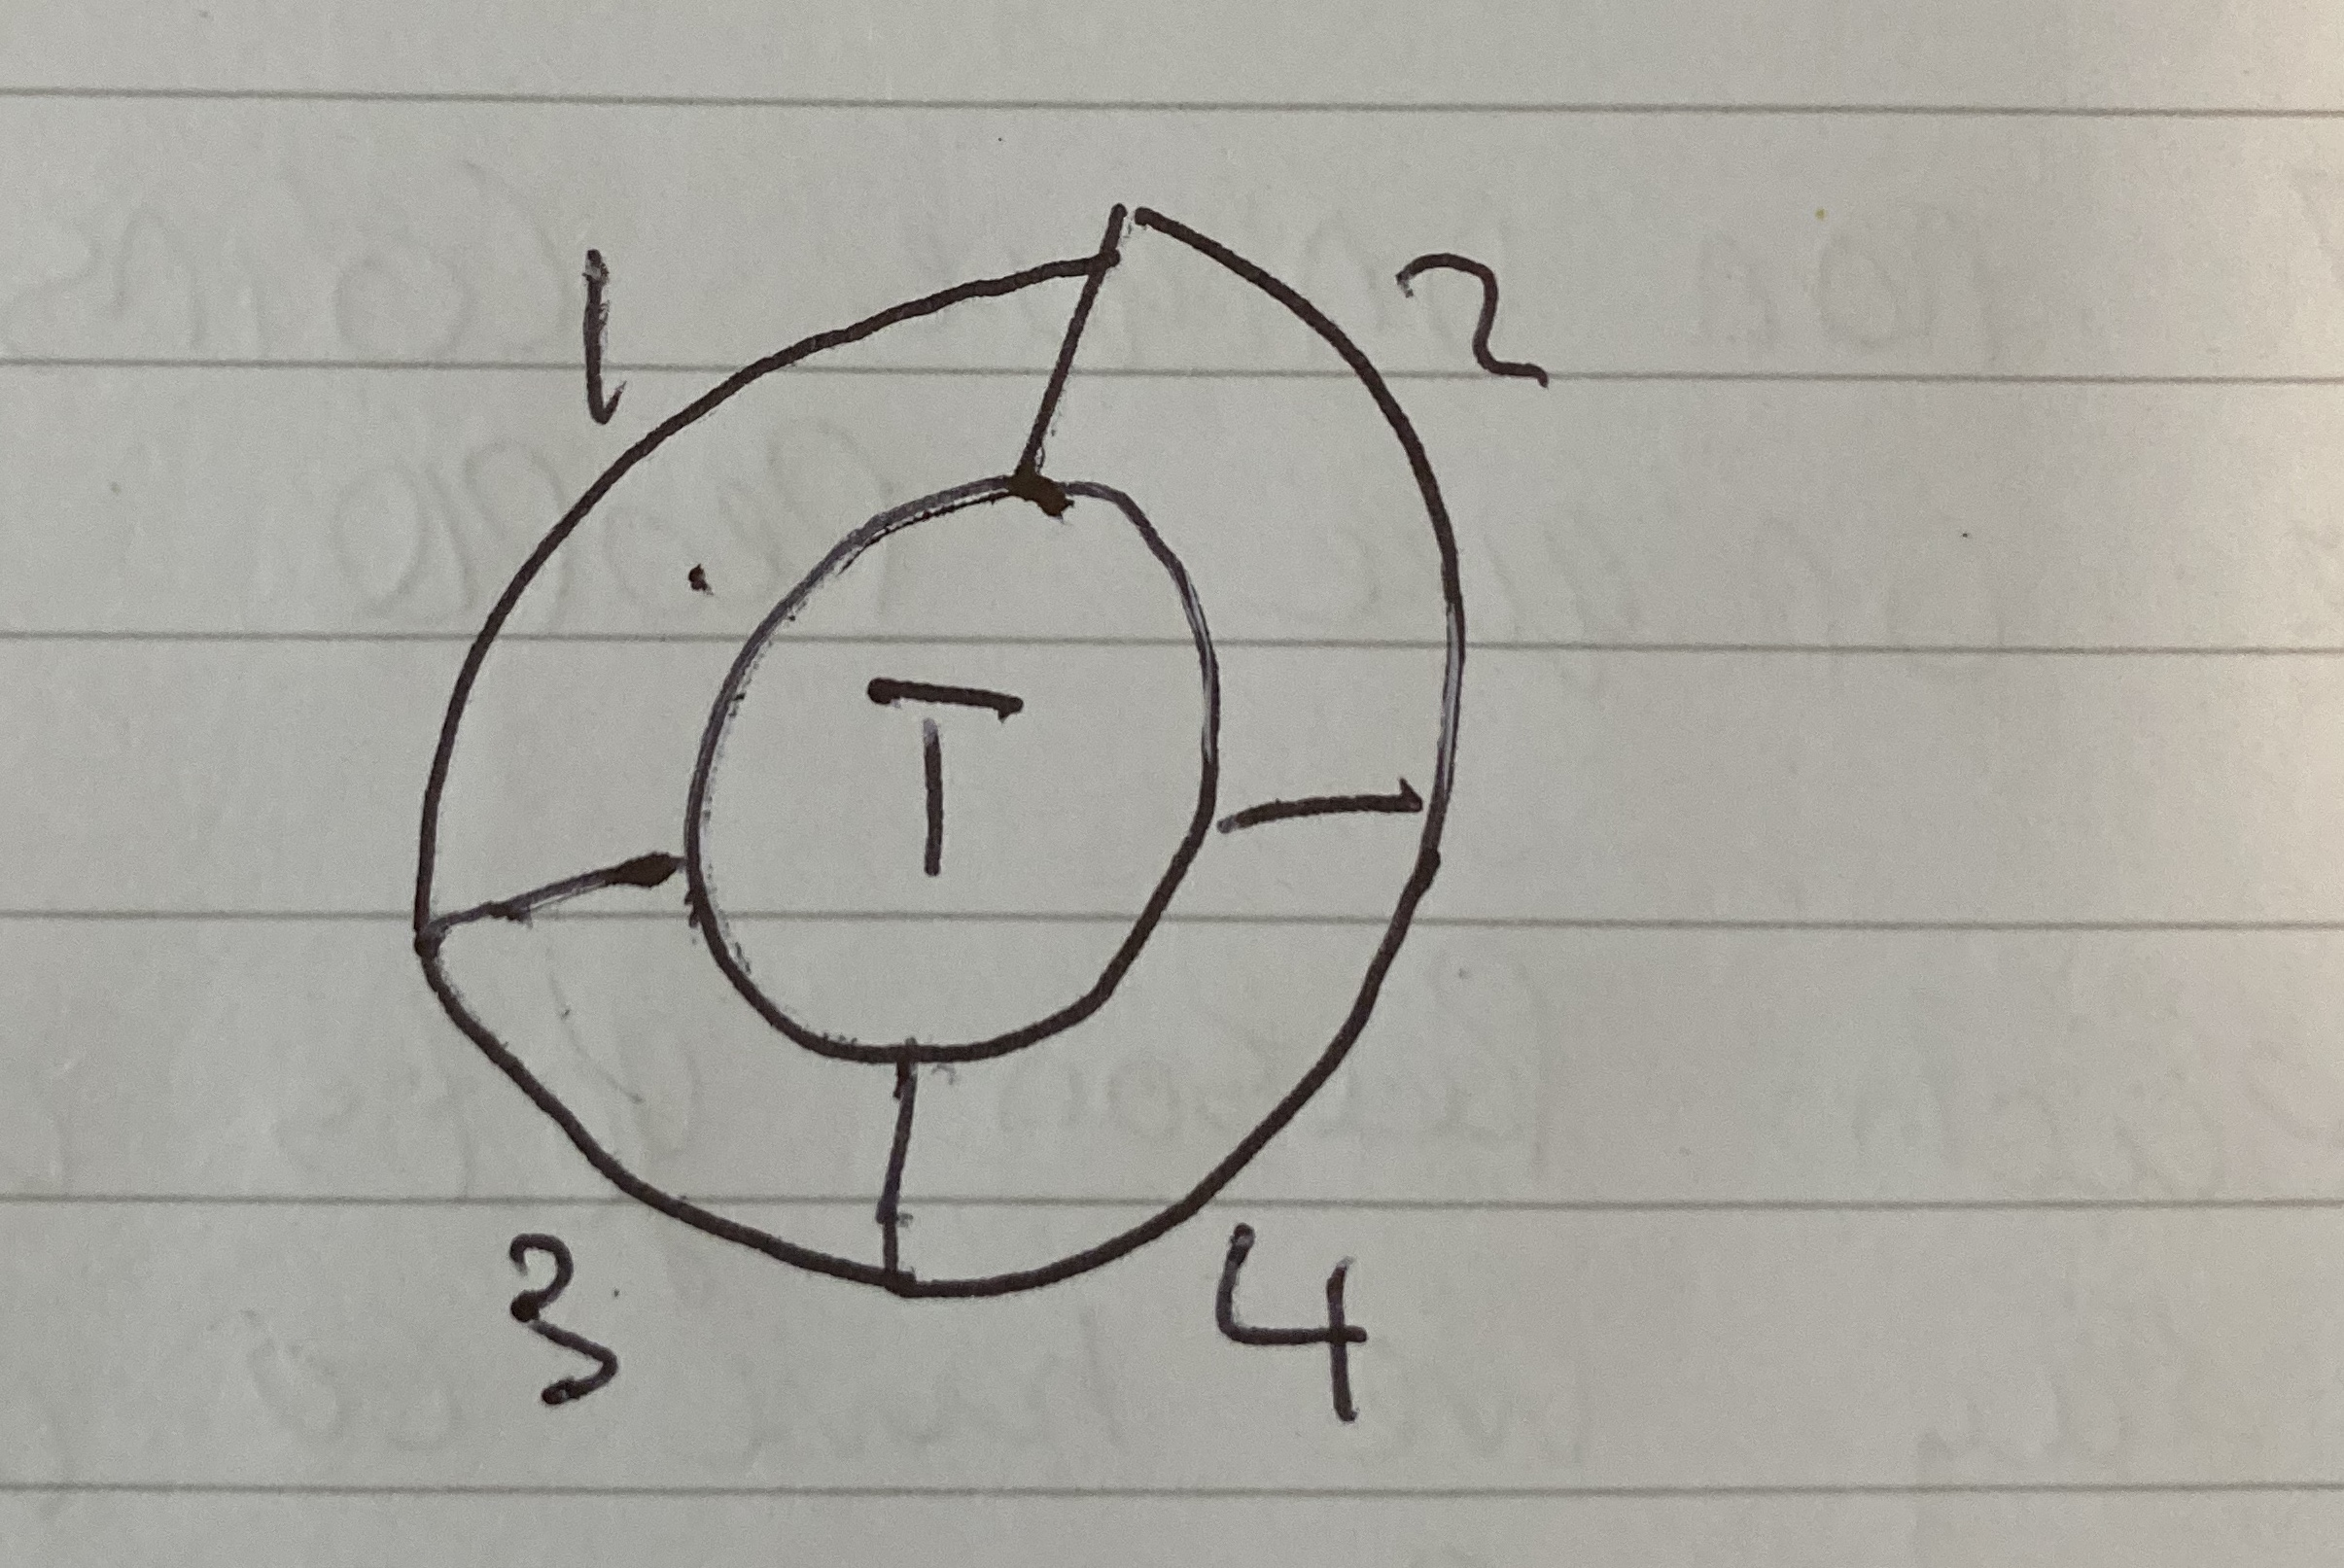
\includegraphics[width=8cm]{table.jpg}
\caption{Table for Question 3. Circular table to fit 4 people round. }
\end{figure}
For this question there can be multiple answers depending on how you view the problem. If the seats are distinguishable then we can view the problem as a mapping of the group $S_4$ where we map People $\rightarrow$ Seats. In this case there are 
$$ |S_4| = N! = 4! = 24! $$
Configurations. We can also view the problem as it \underline{does} matter who sits next to who, including worrying about which side as well:
$$ 1 \rightarrow (2,3),(3,2) $$
$$ 2 \rightarrow (1,4),(4,1) $$
$$ 3 \rightarrow (1,4),(4,1) $$ 
$$ 4 \rightarrow (3,2),(2,3) $$ 
Noticing that we can discount two of them that are not unique we have 6 configurations ($3!$) where it does matter which side you sit on. If we do not care about which side the people sit on then there are only 3 configurations. This is equivalent to looking at the group $\mathbb{Z}_4$, symmetric group and $\mathbb{Z}_2 $ symmetric flip group. 

\item Question 4.
\\
Recognising that there are 7 non-unique coins and 3 unique people as wella s the fact that each person gets at least 1 coin, we can say we have to distribute $7-3$ coins to 3 people. 
\\
There are 4 ways of distributing these 4 coins which I will try to illustate in the table below
\\
\begin{table}[h]
     \centering
     \begin{tabular}{ll|l|l|l|l|}
     \cline{3-6}
                             &   & 3+1 & 2+2 & 2+1+1 & 4    \\ \hline
     \multicolumn{1}{|l|}{A} & i & iii & ii  & ii    & iiii \\ \hline
     \multicolumn{1}{|l|}{B} & i & i   & ii  & ii    & 0    \\ \hline
     \multicolumn{1}{|l|}{C} & i & 0   & 0   & i     & 0    \\ \hline
     \end{tabular}
     \caption{Table illustrating the different ways 4 coins can be distributed between 3 players given that the must have at least 1 coin. One i is equivalent to 1 coin using tally notation. Of course the way these different coins are distributed can be to different people as on the table, this was just an example.}
     \end{table}
\\
Note that $1+1+1+1$ is always a way of distributing 4 coins but not between 3 people without crossover of other ways. 
\\
$4, 2+2,$ and $2+1+1$ can be distributed 3 ways. $3+1$ can be distributed 6 ways. This is the number of unique situations where each person is unique but the coins are not. 
\\ 
Therefore the total number of ways these can be distributed is 
$$ 3+3+3+6 =15 $$
For each person getting a different number of coins and at least one coin then the only option is to distribute the coins in a $1:2:4$ fashion (Different to other permutations such as $4:2:1$ as people are unique). As the people are unique this gives $3!$ different ways which is 6. 

\item Question 5.
$$ U(n) = \{A \in GL(n,\mathbb{C}) | A^\dagger A = \mathbbm{1}_n\} $$
The $\dagger$ notation meaning $A^\dagger = (A^*)^\dagger $. We can show that $U(n)$ inherits associativity from the group $GL(n,\mathbb{C})$ as $\mathbbm{1}^\dagger \mathbbm{1} = \mathbbm{1}$ so $ \mathbbm{1} \in U(n)$ (The identity of the subgroup is the identity of the group).
\\ Let us confirm closure in $U(n)$
$$ A,B \in U(n) \rightarrow (AB)^\dagger (AB) $$
$$ (AB)^\dagger (AB) = B^\dagger A^\dagger AB = B^\dagger B^\dagger = mathbbm{1} $$
$$ \therefore AB \in U(n) $$
Let us confirm that it is invertable: 
$$ A \in U(n) \rightarrow (A^\dagger)^\dagger A^\dagger = AA^\dagger = \mathbbm{1} $$
Since both matrices coincide and A is unitary 
$$ \therefore A^\dagger \in U(n) $$
We can put these two together in a neater definition of a subgroup and say that 
$$ A,B \in U(n) \rightarrow AB^\dagger \in U(n) $$ 
$U(n)$ is this a subgroup. It is trivial to show that $U(n)$ is a proper subgroup as 
$$ U(n) \neq GL(n,\mathbb{C}) $$
In fact it is a non trivial proper subgroup as $\{e\} \neq U(n)$. 
\\
For the dimension dim $U(n) = n^2$ we notice that as $U(n)$ is the unitary matrix we can write it as 
$$ U(n) = \exp(iH) $$
Where $H$ is a hermitian matrix meaning that is conjugate transpose is equal to itself $H^\dagger = H$. A hermitian matrix of size $n$ will always have $n^2 -n$ non diagonal elements which are complex. This can be easily seen in the case of the Pauli matrices. Only half of these elements are independent as the other half contains elements which are complex conjugates. However as these are complex we say that there are $n^2 -n$ real independent parameters on the off-diagonal. The diagonal elements of a hermitian matrix are real, meaning that 
$$ dim U(n) = n^2 - n +n = n^2 $$ 
$$ dim U(n) = n^2 $$ 
\end{enumerate}


\end{document}
